\section{FTK}

\begin{frame}[fragile]
  \frametitle{FTK}
  \begin{itemize}
  \item We tried to use FTK as a feature detector to compare the original and lossy data
  \item As a distance, we use normalized difference of the number of local maxima
  \item Next slide shows how this distance depends on the tolerance that is a parameter
    for each compressor
  \item ZFP and MGARD have only one input parameter to control the compression
  \item SZ can use several kinds of tolerance parameters, here by ``tolerance'' we mean the default one: \verb|pw_relBoundRatio|
  \end{itemize}
\end{frame}

\subsection{Distance}
\begin{frame}[fragile]
  \frametitle{FTK: distance}
  
  There is no clear correlation between tolerance and FTK distance
  
  \begin{center}
    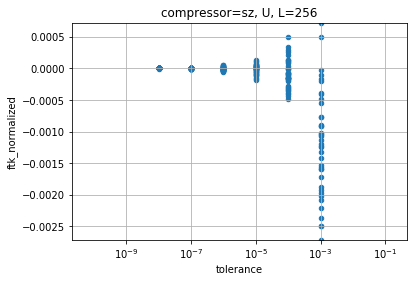
\includegraphics[width=3.7cm]{graphs/ndistance_sz_U.png}
    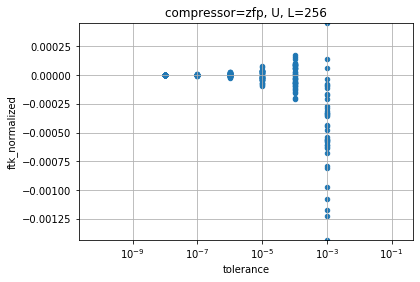
\includegraphics[width=3.7cm]{graphs/ndistance_zfp_U.png}
    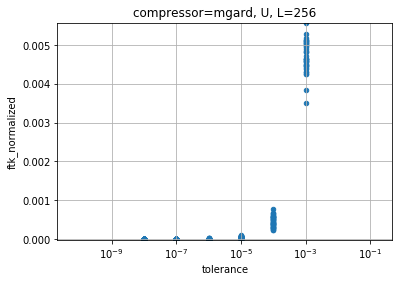
\includegraphics[width=3.7cm]{graphs/ndistance_mgard_U.png}
    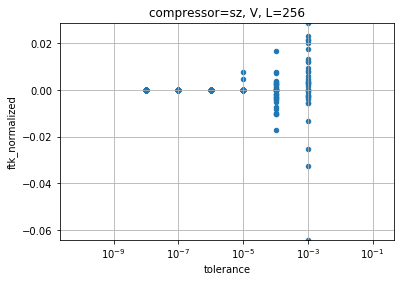
\includegraphics[width=3.7cm]{graphs/ndistance_sz_V.png}
    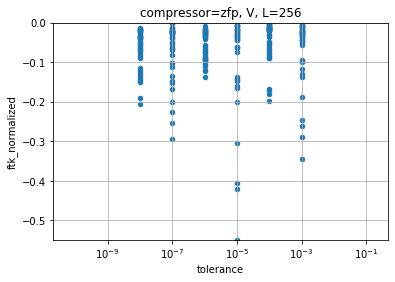
\includegraphics[width=3.7cm]{graphs/ndistance_zfp_V.png}
    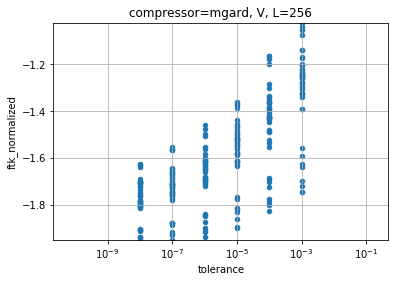
\includegraphics[width=3.7cm]{graphs/ndistance_mgard_V.png}    
  \end{center}
\end{frame}

\subsection{ZChecker}
\begin{frame}[fragile]
  \frametitle{FTK: ZChecker measurements}

  Varios ZChecker's measurements behave as expected

  \begin{center}
    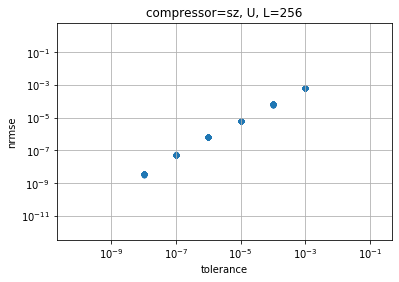
\includegraphics[width=3.7cm]{graphs/rmse_sz_U.png}
    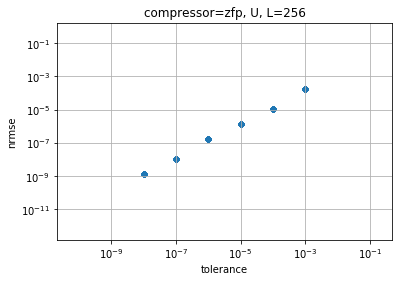
\includegraphics[width=3.7cm]{graphs/rmse_zfp_U.png}
    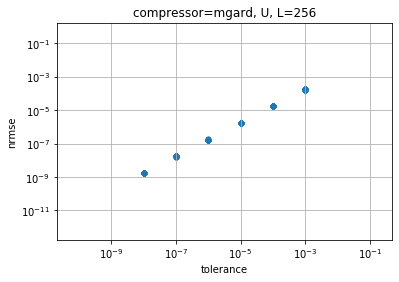
\includegraphics[width=3.7cm]{graphs/rmse_mgard_U.png}
    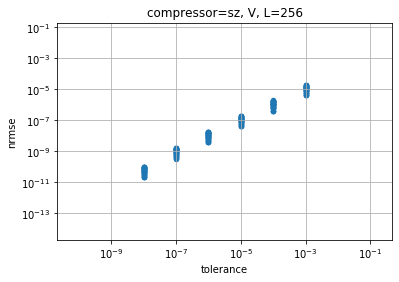
\includegraphics[width=3.7cm]{graphs/rmse_sz_V.png}
    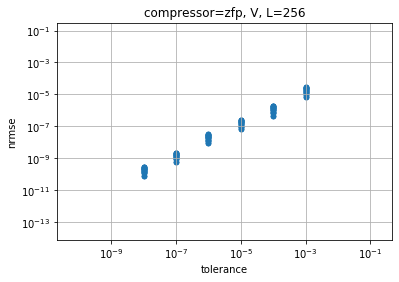
\includegraphics[width=3.7cm]{graphs/rmse_zfp_V.png}
    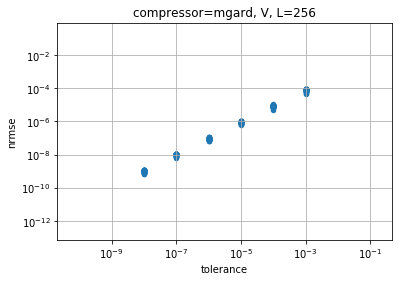
\includegraphics[width=3.7cm]{graphs/rmse_mgard_V.png}        
  \end{center}

\end{frame}

\subsection{Number of maxima for $noise = 10^{-2}$}
\subsubsection{SZ}
\begin{frame}[fragile]
  \frametitle{FTK: number of maxima for $noise = 10^{-2}$, SZ }

{\tiny
\begin{table}[H]
\centering
\begin{tabular}{|r|r|r|r|r|}
\hline
tolerance &         number of max, original &         number of max, lossy &       difference & normalized difference \\
\hline
  1.0e-08 &           828279 &        828279 &             0.0 &       0.00e+00 \\
\hline
  1.0e-07 &           825165 &        825166 &            -1.0 &      -1.21e-06 \\
\hline
  1.0e-06 &           825966 &        825996 &           -30.0 &      -3.63e-05 \\
\hline
  1.0e-05 &           824939 &        825007 &           -68.0 &      -8.24e-05 \\
\hline
  1.0e-04 &           827345 &        827418 &           -73.0 &      -8.82e-05 \\
\hline
  1.0e-03 &           824677 &        825416 &          -739.0 &      -8.96e-04 \\
\hline
\end{tabular}
\caption{SZ, U, $step = 1000$, $noise = 10^{-2}$}
\label{sz_u_table}
\end{table}
}

{\tiny
Notice: the number of maxima in the original data above is only 20 times smaller than the total number of points in the volume.
}

{\tiny
\begin{table}[H]
\centering
\begin{tabular}{|r|r|r|r|r|}
\hline
tolerance &         number of max, original &         number of max, lossy &       difference & normalized difference \\
\hline

  1.0e-08 &              981 &           981 &             0.0 &       0.00e+00 \\
\hline
  1.0e-07 &             1004 &          1004 &             0.0 &       0.00e+00 \\
\hline
  1.0e-06 &              917 &           917 &             0.0 &       0.00e+00 \\
\hline
  1.0e-05 &             1003 &          1003 &             0.0 &       0.00e+00 \\
\hline
  1.0e-04 &              987 &           985 &             2.0 &       2.03e-03 \\
\hline
  1.0e-03 &              941 &           942 &            -1.0 &      -1.06e-03 \\
\hline
\end{tabular}
\caption{SZ, V, $step = 1000$, $noise = 10^{-2}$}
\label{sz_v_table}
\end{table}
}

  
\end{frame}


\begin{frame}[fragile]
  \frametitle{FTK: number of maxima for $noise = 10^{-2}$, SZ }

  \begin{itemize}
  \item For $V$ the number of maxima is of reasonable size and almost identical between the original
    and lossy data; a small difference appears only at high tolerance $10^{-4}$
  \item The difference between the graphs and the tables is coming from two sources:
    \begin{itemize}
    \item In the tables only the last checkpoint is shown while on the graph all 10 checkpoints
    \item In the tables the results shown only for 64 MPI ranks for Gray-Scott and ZChecker (this experiment was done on theta)
      while on the graphs 4 combinations of $(32, 64)$ ranks are tried
    \end{itemize}
  \end{itemize}
\end{frame}

\subsubsection{ZFP}
\begin{frame}[fragile]
  \frametitle{FTK: number of maxima for $noise = 10^{-2}$, ZFP }

  {\tiny
    \begin{table}[H]
      \centering
      \begin{tabular}{|r|r|r|r|r|}
        \hline
        tolerance &         number of max, original &         number of max, lossy &       difference & normalized difference \\
        \hline
        1.0e-08 &           825854 &        825854 &             0.0 &       0.00e+00 \\
        \hline
        1.0e-07 &           827774 &        827777 &            -3.0 &      -3.62e-06 \\
        \hline
        1.0e-06 &           826774 &        826766 &             8.0 &       9.68e-06 \\
        \hline
        1.0e-05 &           826603 &        826629 &           -26.0 &      -3.15e-05 \\
        \hline
        1.0e-04 &           825891 &        825910 &           -19.0 &      -2.30e-05 \\
        \hline
        1.0e-03 &           826406 &        826549 &          -143.0 &      -1.73e-04 \\
        \hline
      \end{tabular}
      \caption{ZFP, U, $step = 1000$, $noise = 10^{-2}$}
      \label{zfp_u_table}
    \end{table} 
  }

  {\tiny
    \begin{table}[H]
      \centering
      \begin{tabular}{|r|r|r|r|r|}
        \hline
        tolerance &         number of max, original &         number of max, lossy &       difference & normalized difference \\
        \hline
        
        1.0e-08 &              914 &           933 &           -19.0 &      -2.06e-02 \\
        \hline
        1.0e-07 &             1064 &          1092 &           -28.0 &      -2.60e-02 \\
        \hline
        1.0e-06 &             1018 &          1117 &           -99.0 &      -9.29e-02 \\
        \hline
        1.0e-05 &              987 &           994 &            -7.0 &      -7.08e-03 \\
        \hline
        1.0e-04 &              964 &           978 &           -14.0 &      -1.44e-02 \\
        \hline
        1.0e-03 &              975 &           997 &           -22.0 &      -2.23e-02 \\
        \hline
      \end{tabular}
      \caption{ZFP, V, $step = 1000$, $noise = 10^{-2}$}
      \label{zfp_v_table}
    \end{table}
  }

  {\tiny
    While the results for $U$ are similar to those of SZ, the results for $V$ show no clear correlation between the number of maxima and the tolerance, and this is correctly reflected in more or less constant absolute value of distance
  }
\end{frame}



\subsubsection{MGARD}
\begin{frame}[fragile]
  \frametitle{FTK: number of maxima for $noise = 10^{-2}$, MGARD }

  {\tiny
\begin{table}[H]
\centering
\begin{tabular}{|r|r|r|r|r|}
\hline
tolerance &         number of max, original &         number of max, lossy &       difference & normalized difference \\
\hline

  1.0e-08 &           826506 &        826502 &             4.0 &       4.84e-06 \\
\hline
  1.0e-07 &           825201 &        825204 &            -3.0 &      -3.64e-06 \\
\hline
  1.0e-06 &           826299 &        826302 &            -3.0 &      -3.63e-06 \\
\hline
  1.0e-05 &           827031 &        827031 &             0.0 &       0.00e+00 \\
\hline
  1.0e-04 &           824480 &        824156 &           324.0 &       3.93e-04 \\
\hline
  1.0e-03 &           825847 &        821624 &          4223.0 &       5.13e-03 \\
\hline
\end{tabular}
\caption{MGARD, U, $step = 1000$, $noise = 10^{-2}$}
\label{mgard_u_table}
\end{table}

  }

  {\tiny
\begin{table}[H]
\centering
\begin{tabular}{|r|r|r|r|r|}
\hline
tolerance &         number of max, original &         number of max, lossy &       difference & normalized difference \\
\hline
  1.0e-08 &              979 &          9540 &         -8561.0 &      -1.63e+00 \\
\hline
  1.0e-07 &              955 &          7887 &         -6932.0 &      -1.57e+00 \\
\hline
  1.0e-06 &              927 &          6472 &         -5545.0 &      -1.50e+00 \\
\hline
  1.0e-05 &              900 &          4816 &         -3916.0 &      -1.37e+00 \\
\hline
  1.0e-04 &              934 &          3720 &         -2786.0 &      -1.20e+00 \\
\hline
  1.0e-03 &              966 &          3058 &         -2092.0 &      -1.04e+00 \\
\hline
\end{tabular}
\caption{MGARD, V, $step = 1000$, $noise = 10^{-2}$}
\label{mgard_v_table}
\end{table}
  }
 {\tiny
  Notice: for $V$ MGARD lossy data has 10 times more local maxima than the original data and as the tolerance increases,
  the distance decreases which is opposite to what we saw for other compression algorithms. Apparently MGARD introduces its own
  artifacts and the higher the required compression precision, the more artifacts are introduced.
 }
 
\end{frame}


\subsection{Number of maxima for $noise = 0$}
\begin{frame}[fragile]
  \frametitle{FTK: number of maxima for $noise = 0$ }
  \begin{itemize}
  \item Reducing the noise amplitude from $10^{-2}$ to $10^{-5}$ does not significantly change the results:
    still the number of local maxima in the original data for $U$ is only about 20 times less than the number of points in
    the volume - anything, no matter how small, that is larger than its immediate neighbors is considered to be local maxima
  \item Therefore, let us try to turn the noise completely off
  \item We shall consider only two values for tolerance for simplicity
  \end{itemize}
\end{frame}


\begin{frame}[fragile]
  \frametitle{FTK: number of maxima for $noise = 0$ }

  {\tiny
\begin{table}[H]
\centering
\begin{tabular}{|r|r|r|r|r|}
\hline
tolerance &  number of max, original &  number of max, lossy &  difference & normalized difference \\
\hline
  1.0e-08 &               50 &           645 &          -595.0 &      -1.72e+00 \\ \hline
  1.0e-03 &               50 &           452 &          -402.0 &      -1.61e+00 \\  \hline
\end{tabular}
\caption{SZ, U, step=500, $noise=0$}
\label{sz_u_n0}
\end{table}

\begin{table}[H]
\centering
\begin{tabular}{|r|r|r|r|r|}
\hline
tolerance &  number of max, original &  number of max, lossy &  difference & normalized difference \\
\hline
  1.0e-08 &              558 &           614 &           -56.0 &      -9.57e-02 \\ \hline
  1.0e-03 &              558 &           551 &             7.0 &       1.27e-02 \\ \hline
\end{tabular}
\caption{SZ, V, step=500, $noise=0$}
\label{sz_v_n0}
\end{table}

 \begin{table}[H]
\centering
\begin{tabular}{|r|r|r|r|r|}
\hline
tolerance &  number of max, original &  number of max, lossy &  difference & normalized difference \\
\hline 
  1.0e-08 &               50 &           219 &          -169.0 &      -1.27e+00 \\ \hline
  1.0e-03 &               50 &           235 &          -185.0 &      -1.31e+00 \\ \hline
\end{tabular}
\caption{ZFP, U, step=500, $noise=0$}
\label{zfp_u_n0}
\end{table}

\begin{table}[H]
\centering
\begin{tabular}{|r|r|r|r|r|}
\hline
tolerance &  number of max, original &  number of max, lossy &  difference & normalized difference \\
\hline 
  1.0e-08 &              558 &           579 &           -21.0 &      -3.70e-02 \\ \hline
  1.0e-03 &              558 &           617 &           -59.0 &      -1.01e-01 \\ \hline
\end{tabular}
\caption{ZFP, V, step=500, $noise=0$}
\label{zfp_v_n0}
\end{table}

 



  }

  
\end{frame}


\begin{frame}[fragile]
  \frametitle{FTK: number of maxima for $noise = 0$ }

  {\tiny

 \begin{table}[H]
\centering
\begin{tabular}{|r|r|r|r|r|}
\hline
tolerance &  number of max, original &  number of max, lossy &  difference & normalized difference \\
\hline 

  1.0e-08 &               50 &          4687 &         -4637.0 &      -1.96e+00 \\ \hline
  1.0e-03 &               50 &          1224 &         -1174.0 &      -1.85e+00 \\ \hline
\end{tabular}
\caption{MGARD, U, step=500, $noise=0$}
\label{mgard_u_n0}
\end{table}

\begin{table}[H]
\centering
\begin{tabular}{|r|r|r|r|r|}
\hline
tolerance &  number of max, original &  number of max, lossy &  difference & normalized difference \\
\hline 

  1.0e-08 &              558 &          6480 &         -5922.0 &      -1.68e+00 \\ \hline
  1.0e-03 &              558 &          1860 &         -1302.0 &      -1.08e+00 \\ \hline
\end{tabular}
\caption{MGARD, V, step=500, $noise=0$}
\label{mgard_v_n0}
\end{table}

  }


  \begin{itemize}
  \item While setting $noise = 0$ got rid of unmanageable number of local maxima in the original data, it did not address
    compression/decompression artifacts generated in the lossy data
  \item Hanqi suggested to try to use Gaussian filtering to precondition data before applying FTK - almost finished implementing it
  \end{itemize}
  
\end{frame}
